\section{Vector Error Regression}
\subsection{Algoritmo Propuesto}
\subsection{Diagrama de Clases}

La implementación fue realizada en Python, usando principalmente las bibliotecas:
\begin{itemize}
 \item Pandas: biblioteca para manipulación y análisis de datos. \footnote{\url{http://pandas.pydata.org}}
 \item Statsmodels: módulo que permite explorar data, estimar modelos y test
estadísticos. \footnote{\url{}}
 \item Numpy: paquete de computación científica en Python, provee estructuras
de datos y funciones de álgebra lineal entre otras cosas.
\footnote{\url{http://www.numpy.org}}
 \item Scikit.CUDA: provee interfaces a un set de funciones de CUDA, cuBLAS y
otras bibliotecas. La idea es poder ejecutar funciones de cuda desde python a
través de wrappers. \footnote{\url{http://scikits.appspot.com/cuda}}
\end{itemize}

Basándose en esas bibliotecas y otras más, se crearon 3 clases mostrados en la
figura \ref{fig:class_diagram}:
\begin{itemize}
 \item Util: provee métodos generales utilizados por las otras 2 clases.
 \item Reader: clase que lee los datos ticks desde archivos CSV descargados
desde dukascopy, provee funciones para juntar monedas en la misma estructura de
datos, hacer resampling a cierta frecuencia y normalizar monedas, entre otras
funciones.
 \item Matrix: es la clase es más extensa y contiene los principales métodos
utilizados por los algoritmos, entre ellos la creación de las matrices VAR y
VECM, el update de las matrices optimizado para la ventana deslizante, cálculo
de vectores de integración mediante Johansen, test de estacionaridad usando
Augmented Dicky Fuller, Errores porcentuales, etc.
\end{itemize}

\begin{figure}[h!t]
    \begin{center}
        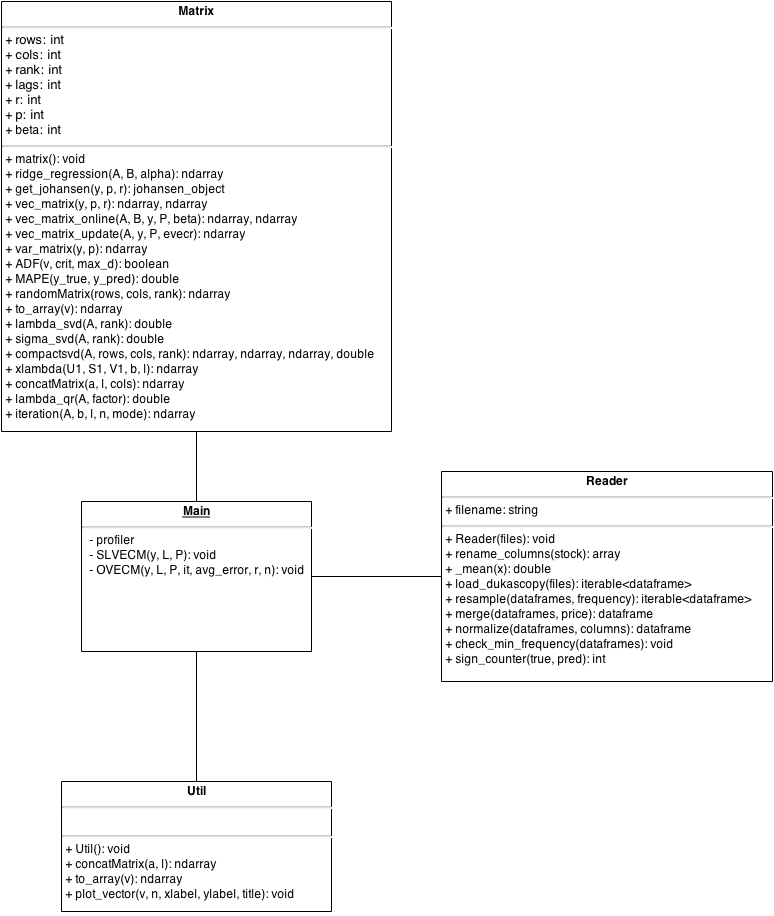
\includegraphics[width=0.8\textwidth]{images/class_diagram.png}
        \caption{Diagrama de Clases}
        \label{fig:class_diagram}
    \end{center}
\end{figure}

%\section{Esquema de paralelizacion}
%\subsection{BLAS - cuBLAS}
\section{Métodos a paralelizar}
